\chapter{Результаты и их обсуждение}
\label{ch:results}

\section{Экспериментальная установка}

    %Почему именно такая установка, что она позволяет измерить
    В работе использовалась установка с цилиндрической симметрией. Температура стенок цилиндра поддерживалась постоянной. Нить нагрева поместили на оси цилиндра. Такая установка позволила считать поток тепла направленным строго радиально и рассматривать изменение температуры только в этом направлении.
    
    \begin{figure}[ht]
    \centering
        
\includegraphics[width = 0.7\textwidth]{img/ustanovka.png}
        \begin{center}
        Рис. 1. Схема установки. $L$ - высота цилиндра, $r_0$ - радиус цилиндра, $r_1$ - радиус нити. Эти параметры использовались при нахождении полного потока тепла через цилиндр. Поток тепла рассматривался только в радиальном направлении. %(полностью описание) для чего, что на рисунке
        \end{center}
    \end{figure}
    
    На рис. 1 приведена схема установки (См. Приложение А)

    %Само описание установки в приложение. Технику измерения температуры тоже в приложение.

\section{Методика измерений}
    
    Известно, что поток тепла выражается из закона Фурье, в котором говорится, что плотность потока энергии пропорциональна градиенту температуры. В случае цилиндрической симметрии получается следующее выражение (вывод см. в приложении Б).
    %(можно ссылку на параграф)

    \begin{align}
        Q &= \dfrac{2 \pi L}{\ln \dfrac{r_0}{r_1}} k  \cdot \Delta T \label{Q}
    \end{align}

\section{Обработка результатов измерений}

    По экспериментальным данным определили коэффициент зависимости сопротивления от температуры $\frac{dR}{dT}$ и угловые коэффициенты нагрузочных прямых $\frac{dR}{dQ}$ (Методики измерения и расчёты см. в Приложении Г и Приложении Д). Используя эти данные, нашли зависимость выделяющейся на нити мощности $Q$ от её перегрева $\Delta T$ относительно стенок из выражения:
    
    \[\frac{dQ}{d(\Delta T)} = \frac{dR}{dT}/\frac{dR}{dQ}.\]

    \begin{figure}[ht]
        \center{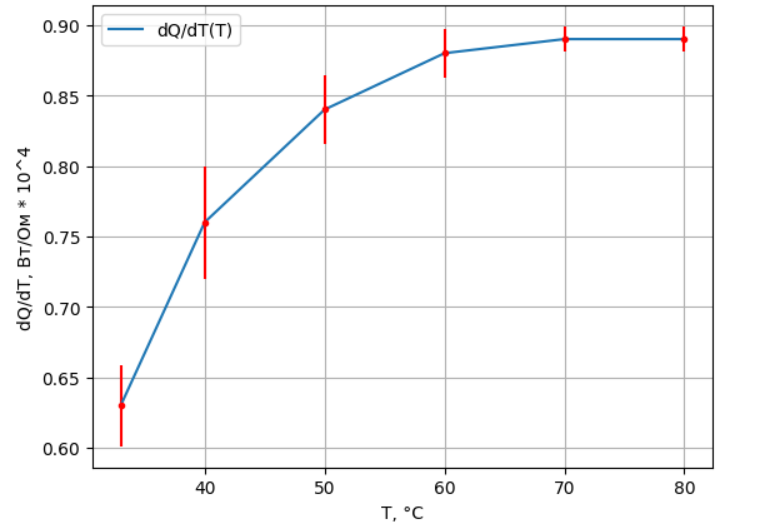
\includegraphics[scale=0.5]{img/dQdT(T).png}}
        \begin{center}            
        Рис. 2. График зависимости $\frac{dQ}{dT} (T)$. Красным цветом выделены экспериментальные точки. Синяя линия проведена для удобства восприятия.
        \end{center}
        \label{kT_graph}
    \end{figure}

%На графике $R_{\text{н}}(Q)$ сразу температура, а не сопротивление. + Точки экспериментальные. + погрешности на графике. (Вт/Ом * 10^4);

    Для каждой температуры определили $k$ - коэффициент теплопроводности воздуха по формуле:
    \[k = \frac{dQ}{dT} \frac{1}{2 \uppi L} \ln{\frac{r_2}{r_1}}.\]

    Результаты показаны на графике (см. рис. 3).
    
    \begin{figure}[ht]
        \center{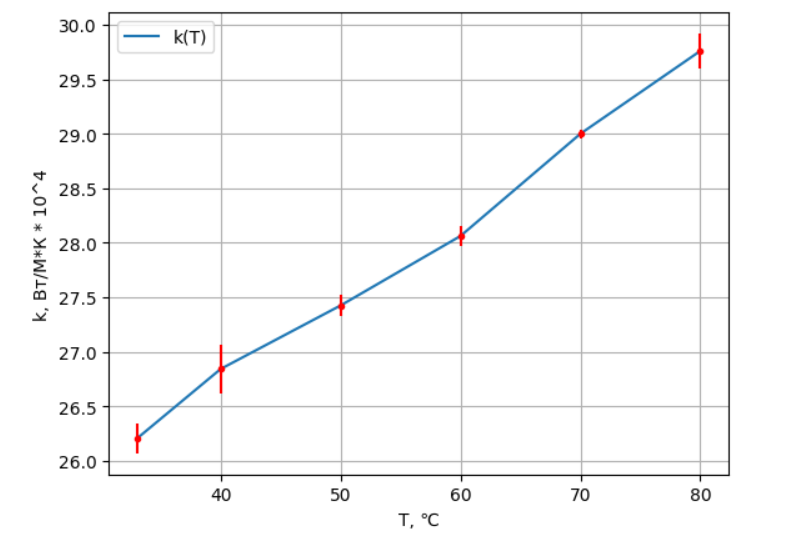
\includegraphics[scale=0.5]{img/k(T).png}}
        \begin{center}            
        Рис. 3. График зависимости $k (T)$. Красным цветом выделены экспериментальные точки. Синяя линия проведена для удобства восприятия % * 10 в степени вынести
        \end{center}
        \label{kT_graph}
    \end{figure}

    Для того, чтобы проверить справедливость утверждения, что $k \sim T^{\beta}$, построили график в двойных логарифмических координатах.

    \begin{figure}[ht]
        \center{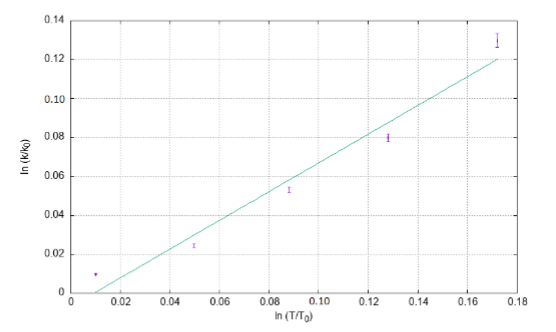
\includegraphics[scale=0.85]{img/lnk.png}}
        \begin{center}            
        Рис. 4. График зависимости $ln (k/k_0) (ln(T/T_0))$. Фиолетовым цветом отмечены точки, полученные в результате измерений. Прямая голубого цвета отражает полученную зависимость $ln (k/k_0) (ln(T/T_0))$.
        \end{center}
        \label{lnk_graph}
    \end{figure}
   
%+ график зависимости k(T)
    
    Из графика на рис. 4. определили показатель степени $\beta$ для формулы $k \sim T^{\beta}$. Коэффициент $\beta = 0.87 \pm 0.03$.
